% Roofline figure for HQC-RISC-V on BPI-F3 (SpacemiT X60)
% Include in thesis with: % Roofline figure for HQC-RISC-V on BPI-F3 (SpacemiT X60)
% Include in thesis with: % Roofline figure for HQC-RISC-V on BPI-F3 (SpacemiT X60)
% Include in thesis with: % Roofline figure for HQC-RISC-V on BPI-F3 (SpacemiT X60)
% Include in thesis with: \input{figures/roofline/roofline.tex}
%
% Requires: pgfplots, pgfplotstable
% Data source: results/hardware/profiling/roofline/roofline_latest.dat
%
% The roofline model plots achieved performance (ops/s) vs arithmetic
% intensity (ops/byte). Two compute ceilings (scalar clmul, vector RVV)
% and one memory bandwidth ceiling (DRAM) are shown.
%
% Operation unit: retired instructions (integer/GF(2) crypto workload).

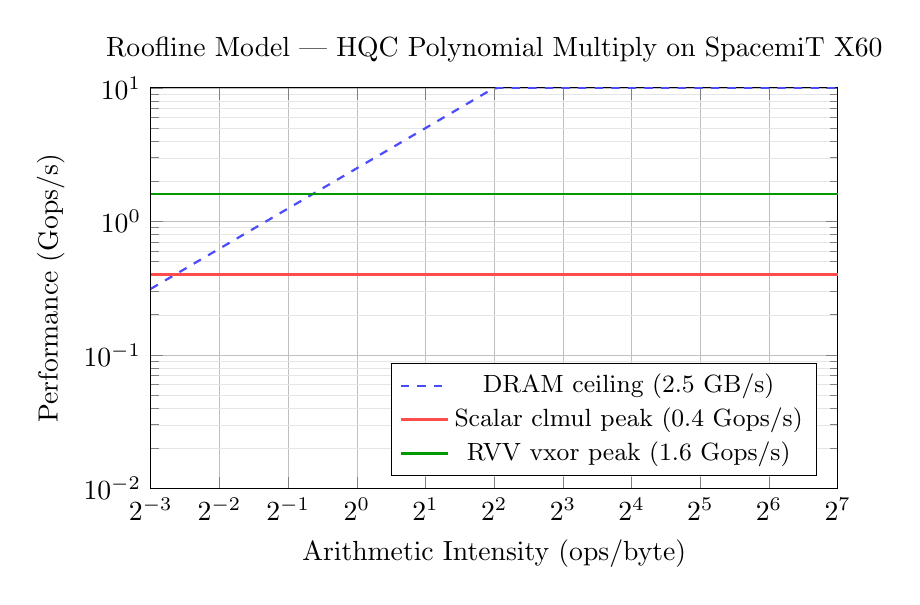
\begin{tikzpicture}
\begin{axis}[
    xlabel={Arithmetic Intensity (ops/byte)},
    ylabel={Performance (Gops/s)},
    xmode=log,
    ymode=log,
    log basis x=2,
    grid=both,
    grid style={line width=.1pt, draw=gray!20},
    major grid style={line width=.2pt, draw=gray!50},
    width=0.85\textwidth,
    height=0.55\textwidth,
    legend pos=south east,
    legend style={font=\small},
    title={Roofline Model --- HQC Polynomial Multiply on SpacemiT X60},
    xmin=0.125, xmax=128,
    ymin=0.01, ymax=10,
]

% ── DRAM bandwidth ceiling (diagonal) ────────────────────────────────────
% Replace <BW_GB_S> with measured peak DRAM BW in GB/s
% The line is: perf = BW × AI (in log-log space: a line with slope 1)
\pgfmathsetmacro{\dramBW}{2.5}  % TODO: replace with measured value
\addplot[domain=0.125:128, samples=100, thick, dashed, blue!70]
    {min(\dramBW * x, 10)};
\addlegendentry{DRAM ceiling (\pgfmathprintnumber{\dramBW} GB/s)}

% ── Scalar compute ceiling (horizontal) ─────────────────────────────────
% Replace <SCALAR_GOPS> with measured peak scalar ops/s / 1e9
\pgfmathsetmacro{\scalarPeak}{0.4}  % TODO: replace with measured value
\addplot[domain=0.125:128, samples=2, thick, red!70]
    {\scalarPeak};
\addlegendentry{Scalar clmul peak (\pgfmathprintnumber{\scalarPeak} Gops/s)}

% ── Vector compute ceiling (horizontal) ──────────────────────────────────
% Replace <VECTOR_GOPS> with measured peak vector ops/s / 1e9
\pgfmathsetmacro{\vectorPeak}{1.6}  % TODO: replace with measured value
\addplot[domain=0.125:128, samples=2, thick, green!60!black]
    {\vectorPeak};
\addlegendentry{RVV vxor peak (\pgfmathprintnumber{\vectorPeak} Gops/s)}

% ── Data points ──────────────────────────────────────────────────────────
% Load from the generated .dat file
% Uncomment after running gen_roofline.py:
%
% \addplot[only marks, mark=*, mark size=2pt, red!80!black]
%     table[x=ai, y=achieved_gops, restrict expr to domain=
%         {\thisrow{variant}}{scalar_ref:scalar_ref}]
%     {figures/roofline/roofline_latest.dat};
% \addlegendentry{scalar\_ref}
%
% \addplot[only marks, mark=square*, mark size=2pt, orange!80!black]
%     table[x=ai, y=achieved_gops, restrict expr to domain=
%         {\thisrow{variant}}{scalar_zb:scalar_zb}]
%     {figures/roofline/roofline_latest.dat};
% \addlegendentry{scalar\_zb}
%
% \addplot[only marks, mark=triangle*, mark size=3pt, green!60!black]
%     table[x=ai, y=achieved_gops, restrict expr to domain=
%         {\thisrow{variant}}{vector_rvv:vector_rvv}]
%     {figures/roofline/roofline_latest.dat};
% \addlegendentry{vector\_rvv}

\end{axis}
\end{tikzpicture}

%
% Requires: pgfplots, pgfplotstable
% Data source: results/hardware/profiling/roofline/roofline_latest.dat
%
% The roofline model plots achieved performance (ops/s) vs arithmetic
% intensity (ops/byte). Two compute ceilings (scalar clmul, vector RVV)
% and one memory bandwidth ceiling (DRAM) are shown.
%
% Operation unit: retired instructions (integer/GF(2) crypto workload).

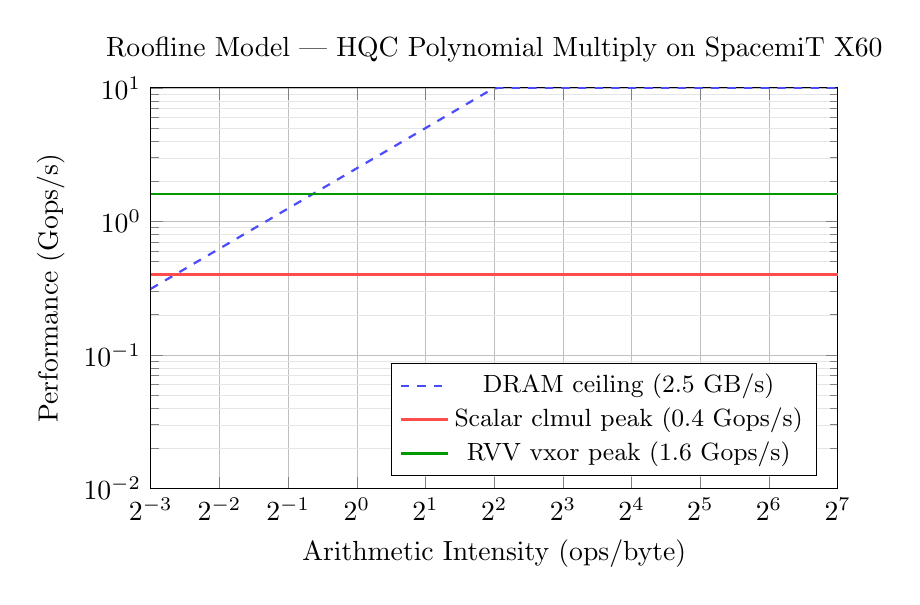
\begin{tikzpicture}
\begin{axis}[
    xlabel={Arithmetic Intensity (ops/byte)},
    ylabel={Performance (Gops/s)},
    xmode=log,
    ymode=log,
    log basis x=2,
    grid=both,
    grid style={line width=.1pt, draw=gray!20},
    major grid style={line width=.2pt, draw=gray!50},
    width=0.85\textwidth,
    height=0.55\textwidth,
    legend pos=south east,
    legend style={font=\small},
    title={Roofline Model --- HQC Polynomial Multiply on SpacemiT X60},
    xmin=0.125, xmax=128,
    ymin=0.01, ymax=10,
]

% ── DRAM bandwidth ceiling (diagonal) ────────────────────────────────────
% Replace <BW_GB_S> with measured peak DRAM BW in GB/s
% The line is: perf = BW × AI (in log-log space: a line with slope 1)
\pgfmathsetmacro{\dramBW}{2.5}  % TODO: replace with measured value
\addplot[domain=0.125:128, samples=100, thick, dashed, blue!70]
    {min(\dramBW * x, 10)};
\addlegendentry{DRAM ceiling (\pgfmathprintnumber{\dramBW} GB/s)}

% ── Scalar compute ceiling (horizontal) ─────────────────────────────────
% Replace <SCALAR_GOPS> with measured peak scalar ops/s / 1e9
\pgfmathsetmacro{\scalarPeak}{0.4}  % TODO: replace with measured value
\addplot[domain=0.125:128, samples=2, thick, red!70]
    {\scalarPeak};
\addlegendentry{Scalar clmul peak (\pgfmathprintnumber{\scalarPeak} Gops/s)}

% ── Vector compute ceiling (horizontal) ──────────────────────────────────
% Replace <VECTOR_GOPS> with measured peak vector ops/s / 1e9
\pgfmathsetmacro{\vectorPeak}{1.6}  % TODO: replace with measured value
\addplot[domain=0.125:128, samples=2, thick, green!60!black]
    {\vectorPeak};
\addlegendentry{RVV vxor peak (\pgfmathprintnumber{\vectorPeak} Gops/s)}

% ── Data points ──────────────────────────────────────────────────────────
% Load from the generated .dat file
% Uncomment after running gen_roofline.py:
%
% \addplot[only marks, mark=*, mark size=2pt, red!80!black]
%     table[x=ai, y=achieved_gops, restrict expr to domain=
%         {\thisrow{variant}}{scalar_ref:scalar_ref}]
%     {figures/roofline/roofline_latest.dat};
% \addlegendentry{scalar\_ref}
%
% \addplot[only marks, mark=square*, mark size=2pt, orange!80!black]
%     table[x=ai, y=achieved_gops, restrict expr to domain=
%         {\thisrow{variant}}{scalar_zb:scalar_zb}]
%     {figures/roofline/roofline_latest.dat};
% \addlegendentry{scalar\_zb}
%
% \addplot[only marks, mark=triangle*, mark size=3pt, green!60!black]
%     table[x=ai, y=achieved_gops, restrict expr to domain=
%         {\thisrow{variant}}{vector_rvv:vector_rvv}]
%     {figures/roofline/roofline_latest.dat};
% \addlegendentry{vector\_rvv}

\end{axis}
\end{tikzpicture}

%
% Requires: pgfplots, pgfplotstable
% Data source: results/hardware/profiling/roofline/roofline_latest.dat
%
% The roofline model plots achieved performance (ops/s) vs arithmetic
% intensity (ops/byte). Two compute ceilings (scalar clmul, vector RVV)
% and one memory bandwidth ceiling (DRAM) are shown.
%
% Operation unit: retired instructions (integer/GF(2) crypto workload).

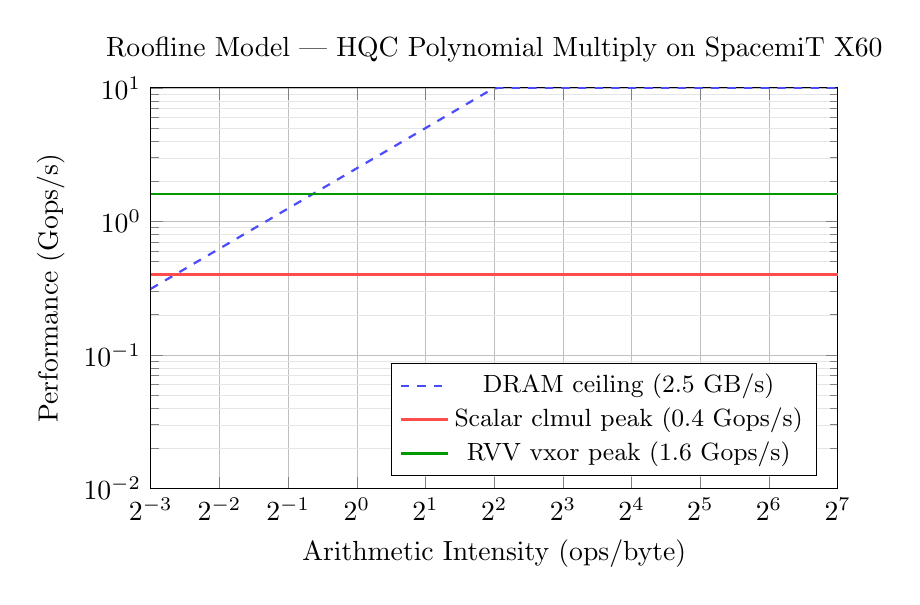
\begin{tikzpicture}
\begin{axis}[
    xlabel={Arithmetic Intensity (ops/byte)},
    ylabel={Performance (Gops/s)},
    xmode=log,
    ymode=log,
    log basis x=2,
    grid=both,
    grid style={line width=.1pt, draw=gray!20},
    major grid style={line width=.2pt, draw=gray!50},
    width=0.85\textwidth,
    height=0.55\textwidth,
    legend pos=south east,
    legend style={font=\small},
    title={Roofline Model --- HQC Polynomial Multiply on SpacemiT X60},
    xmin=0.125, xmax=128,
    ymin=0.01, ymax=10,
]

% ── DRAM bandwidth ceiling (diagonal) ────────────────────────────────────
% Replace <BW_GB_S> with measured peak DRAM BW in GB/s
% The line is: perf = BW × AI (in log-log space: a line with slope 1)
\pgfmathsetmacro{\dramBW}{2.5}  % TODO: replace with measured value
\addplot[domain=0.125:128, samples=100, thick, dashed, blue!70]
    {min(\dramBW * x, 10)};
\addlegendentry{DRAM ceiling (\pgfmathprintnumber{\dramBW} GB/s)}

% ── Scalar compute ceiling (horizontal) ─────────────────────────────────
% Replace <SCALAR_GOPS> with measured peak scalar ops/s / 1e9
\pgfmathsetmacro{\scalarPeak}{0.4}  % TODO: replace with measured value
\addplot[domain=0.125:128, samples=2, thick, red!70]
    {\scalarPeak};
\addlegendentry{Scalar clmul peak (\pgfmathprintnumber{\scalarPeak} Gops/s)}

% ── Vector compute ceiling (horizontal) ──────────────────────────────────
% Replace <VECTOR_GOPS> with measured peak vector ops/s / 1e9
\pgfmathsetmacro{\vectorPeak}{1.6}  % TODO: replace with measured value
\addplot[domain=0.125:128, samples=2, thick, green!60!black]
    {\vectorPeak};
\addlegendentry{RVV vxor peak (\pgfmathprintnumber{\vectorPeak} Gops/s)}

% ── Data points ──────────────────────────────────────────────────────────
% Load from the generated .dat file
% Uncomment after running gen_roofline.py:
%
% \addplot[only marks, mark=*, mark size=2pt, red!80!black]
%     table[x=ai, y=achieved_gops, restrict expr to domain=
%         {\thisrow{variant}}{scalar_ref:scalar_ref}]
%     {figures/roofline/roofline_latest.dat};
% \addlegendentry{scalar\_ref}
%
% \addplot[only marks, mark=square*, mark size=2pt, orange!80!black]
%     table[x=ai, y=achieved_gops, restrict expr to domain=
%         {\thisrow{variant}}{scalar_zb:scalar_zb}]
%     {figures/roofline/roofline_latest.dat};
% \addlegendentry{scalar\_zb}
%
% \addplot[only marks, mark=triangle*, mark size=3pt, green!60!black]
%     table[x=ai, y=achieved_gops, restrict expr to domain=
%         {\thisrow{variant}}{vector_rvv:vector_rvv}]
%     {figures/roofline/roofline_latest.dat};
% \addlegendentry{vector\_rvv}

\end{axis}
\end{tikzpicture}

%
% Requires: pgfplots, pgfplotstable
% Data source: results/hardware/profiling/roofline/roofline_latest.dat
%
% The roofline model plots achieved performance (ops/s) vs arithmetic
% intensity (ops/byte). Two compute ceilings (scalar clmul, vector RVV)
% and one memory bandwidth ceiling (DRAM) are shown.
%
% Operation unit: retired instructions (integer/GF(2) crypto workload).

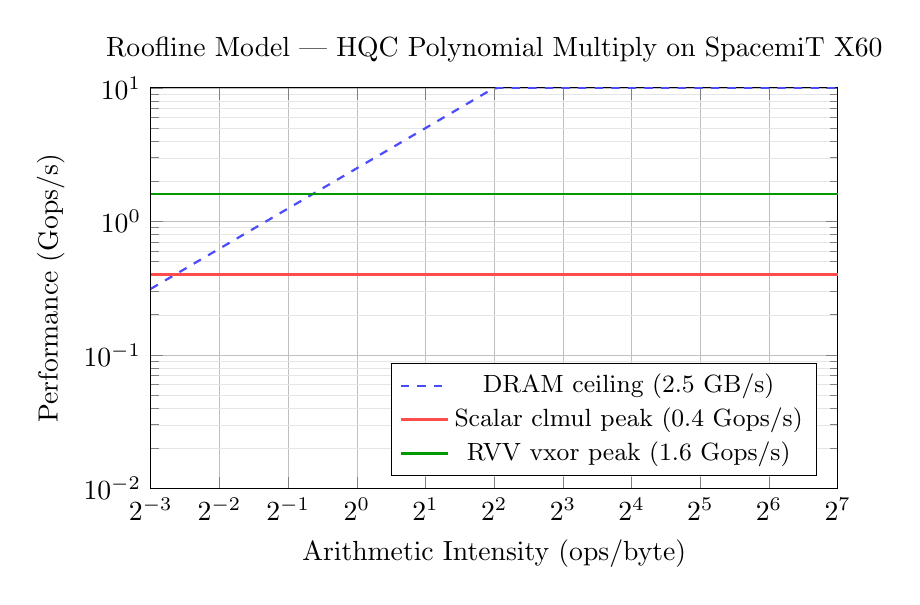
\begin{tikzpicture}
\begin{axis}[
    xlabel={Arithmetic Intensity (ops/byte)},
    ylabel={Performance (Gops/s)},
    xmode=log,
    ymode=log,
    log basis x=2,
    grid=both,
    grid style={line width=.1pt, draw=gray!20},
    major grid style={line width=.2pt, draw=gray!50},
    width=0.85\textwidth,
    height=0.55\textwidth,
    legend pos=south east,
    legend style={font=\small},
    title={Roofline Model --- HQC Polynomial Multiply on SpacemiT X60},
    xmin=0.125, xmax=128,
    ymin=0.01, ymax=10,
]

% ── DRAM bandwidth ceiling (diagonal) ────────────────────────────────────
% Replace <BW_GB_S> with measured peak DRAM BW in GB/s
% The line is: perf = BW × AI (in log-log space: a line with slope 1)
\pgfmathsetmacro{\dramBW}{2.5}  % TODO: replace with measured value
\addplot[domain=0.125:128, samples=100, thick, dashed, blue!70]
    {min(\dramBW * x, 10)};
\addlegendentry{DRAM ceiling (\pgfmathprintnumber{\dramBW} GB/s)}

% ── Scalar compute ceiling (horizontal) ─────────────────────────────────
% Replace <SCALAR_GOPS> with measured peak scalar ops/s / 1e9
\pgfmathsetmacro{\scalarPeak}{0.4}  % TODO: replace with measured value
\addplot[domain=0.125:128, samples=2, thick, red!70]
    {\scalarPeak};
\addlegendentry{Scalar clmul peak (\pgfmathprintnumber{\scalarPeak} Gops/s)}

% ── Vector compute ceiling (horizontal) ──────────────────────────────────
% Replace <VECTOR_GOPS> with measured peak vector ops/s / 1e9
\pgfmathsetmacro{\vectorPeak}{1.6}  % TODO: replace with measured value
\addplot[domain=0.125:128, samples=2, thick, green!60!black]
    {\vectorPeak};
\addlegendentry{RVV vxor peak (\pgfmathprintnumber{\vectorPeak} Gops/s)}

% ── Data points ──────────────────────────────────────────────────────────
% Load from the generated .dat file
% Uncomment after running gen_roofline.py:
%
% \addplot[only marks, mark=*, mark size=2pt, red!80!black]
%     table[x=ai, y=achieved_gops, restrict expr to domain=
%         {\thisrow{variant}}{scalar_ref:scalar_ref}]
%     {figures/roofline/roofline_latest.dat};
% \addlegendentry{scalar\_ref}
%
% \addplot[only marks, mark=square*, mark size=2pt, orange!80!black]
%     table[x=ai, y=achieved_gops, restrict expr to domain=
%         {\thisrow{variant}}{scalar_zb:scalar_zb}]
%     {figures/roofline/roofline_latest.dat};
% \addlegendentry{scalar\_zb}
%
% \addplot[only marks, mark=triangle*, mark size=3pt, green!60!black]
%     table[x=ai, y=achieved_gops, restrict expr to domain=
%         {\thisrow{variant}}{vector_rvv:vector_rvv}]
%     {figures/roofline/roofline_latest.dat};
% \addlegendentry{vector\_rvv}

\end{axis}
\end{tikzpicture}
